\documentclass[]{article}
\usepackage{lmodern}
\usepackage{amssymb,amsmath}
\usepackage{ifxetex,ifluatex}
\usepackage{fixltx2e} % provides \textsubscript
\ifnum 0\ifxetex 1\fi\ifluatex 1\fi=0 % if pdftex
  \usepackage[T1]{fontenc}
  \usepackage[utf8]{inputenc}
\else % if luatex or xelatex
  \ifxetex
    \usepackage{mathspec}
  \else
    \usepackage{fontspec}
  \fi
  \defaultfontfeatures{Ligatures=TeX,Scale=MatchLowercase}
\fi
% use upquote if available, for straight quotes in verbatim environments
\IfFileExists{upquote.sty}{\usepackage{upquote}}{}
% use microtype if available
\IfFileExists{microtype.sty}{%
\usepackage{microtype}
\UseMicrotypeSet[protrusion]{basicmath} % disable protrusion for tt fonts
}{}
\usepackage[margin=1in]{geometry}
\usepackage{hyperref}
\hypersetup{unicode=true,
            pdftitle={Chapter 6: Posterior approximation with the Gibbs sampler},
            pdfauthor={Jesse Mu},
            pdfborder={0 0 0},
            breaklinks=true}
\urlstyle{same}  % don't use monospace font for urls
\usepackage{color}
\usepackage{fancyvrb}
\newcommand{\VerbBar}{|}
\newcommand{\VERB}{\Verb[commandchars=\\\{\}]}
\DefineVerbatimEnvironment{Highlighting}{Verbatim}{commandchars=\\\{\}}
% Add ',fontsize=\small' for more characters per line
\usepackage{framed}
\definecolor{shadecolor}{RGB}{248,248,248}
\newenvironment{Shaded}{\begin{snugshade}}{\end{snugshade}}
\newcommand{\AlertTok}[1]{\textcolor[rgb]{0.94,0.16,0.16}{#1}}
\newcommand{\AnnotationTok}[1]{\textcolor[rgb]{0.56,0.35,0.01}{\textbf{\textit{#1}}}}
\newcommand{\AttributeTok}[1]{\textcolor[rgb]{0.77,0.63,0.00}{#1}}
\newcommand{\BaseNTok}[1]{\textcolor[rgb]{0.00,0.00,0.81}{#1}}
\newcommand{\BuiltInTok}[1]{#1}
\newcommand{\CharTok}[1]{\textcolor[rgb]{0.31,0.60,0.02}{#1}}
\newcommand{\CommentTok}[1]{\textcolor[rgb]{0.56,0.35,0.01}{\textit{#1}}}
\newcommand{\CommentVarTok}[1]{\textcolor[rgb]{0.56,0.35,0.01}{\textbf{\textit{#1}}}}
\newcommand{\ConstantTok}[1]{\textcolor[rgb]{0.00,0.00,0.00}{#1}}
\newcommand{\ControlFlowTok}[1]{\textcolor[rgb]{0.13,0.29,0.53}{\textbf{#1}}}
\newcommand{\DataTypeTok}[1]{\textcolor[rgb]{0.13,0.29,0.53}{#1}}
\newcommand{\DecValTok}[1]{\textcolor[rgb]{0.00,0.00,0.81}{#1}}
\newcommand{\DocumentationTok}[1]{\textcolor[rgb]{0.56,0.35,0.01}{\textbf{\textit{#1}}}}
\newcommand{\ErrorTok}[1]{\textcolor[rgb]{0.64,0.00,0.00}{\textbf{#1}}}
\newcommand{\ExtensionTok}[1]{#1}
\newcommand{\FloatTok}[1]{\textcolor[rgb]{0.00,0.00,0.81}{#1}}
\newcommand{\FunctionTok}[1]{\textcolor[rgb]{0.00,0.00,0.00}{#1}}
\newcommand{\ImportTok}[1]{#1}
\newcommand{\InformationTok}[1]{\textcolor[rgb]{0.56,0.35,0.01}{\textbf{\textit{#1}}}}
\newcommand{\KeywordTok}[1]{\textcolor[rgb]{0.13,0.29,0.53}{\textbf{#1}}}
\newcommand{\NormalTok}[1]{#1}
\newcommand{\OperatorTok}[1]{\textcolor[rgb]{0.81,0.36,0.00}{\textbf{#1}}}
\newcommand{\OtherTok}[1]{\textcolor[rgb]{0.56,0.35,0.01}{#1}}
\newcommand{\PreprocessorTok}[1]{\textcolor[rgb]{0.56,0.35,0.01}{\textit{#1}}}
\newcommand{\RegionMarkerTok}[1]{#1}
\newcommand{\SpecialCharTok}[1]{\textcolor[rgb]{0.00,0.00,0.00}{#1}}
\newcommand{\SpecialStringTok}[1]{\textcolor[rgb]{0.31,0.60,0.02}{#1}}
\newcommand{\StringTok}[1]{\textcolor[rgb]{0.31,0.60,0.02}{#1}}
\newcommand{\VariableTok}[1]{\textcolor[rgb]{0.00,0.00,0.00}{#1}}
\newcommand{\VerbatimStringTok}[1]{\textcolor[rgb]{0.31,0.60,0.02}{#1}}
\newcommand{\WarningTok}[1]{\textcolor[rgb]{0.56,0.35,0.01}{\textbf{\textit{#1}}}}
\usepackage{graphicx,grffile}
\makeatletter
\def\maxwidth{\ifdim\Gin@nat@width>\linewidth\linewidth\else\Gin@nat@width\fi}
\def\maxheight{\ifdim\Gin@nat@height>\textheight\textheight\else\Gin@nat@height\fi}
\makeatother
% Scale images if necessary, so that they will not overflow the page
% margins by default, and it is still possible to overwrite the defaults
% using explicit options in \includegraphics[width, height, ...]{}
\setkeys{Gin}{width=\maxwidth,height=\maxheight,keepaspectratio}
\IfFileExists{parskip.sty}{%
\usepackage{parskip}
}{% else
\setlength{\parindent}{0pt}
\setlength{\parskip}{6pt plus 2pt minus 1pt}
}
\setlength{\emergencystretch}{3em}  % prevent overfull lines
\providecommand{\tightlist}{%
  \setlength{\itemsep}{0pt}\setlength{\parskip}{0pt}}
\setcounter{secnumdepth}{0}
% Redefines (sub)paragraphs to behave more like sections
\ifx\paragraph\undefined\else
\let\oldparagraph\paragraph
\renewcommand{\paragraph}[1]{\oldparagraph{#1}\mbox{}}
\fi
\ifx\subparagraph\undefined\else
\let\oldsubparagraph\subparagraph
\renewcommand{\subparagraph}[1]{\oldsubparagraph{#1}\mbox{}}
\fi

%%% Use protect on footnotes to avoid problems with footnotes in titles
\let\rmarkdownfootnote\footnote%
\def\footnote{\protect\rmarkdownfootnote}

%%% Change title format to be more compact
\usepackage{titling}

% Create subtitle command for use in maketitle
\providecommand{\subtitle}[1]{
  \posttitle{
    \begin{center}\large#1\end{center}
    }
}

\setlength{\droptitle}{-2em}

  \title{Chapter 6: Posterior approximation with the Gibbs sampler}
    \pretitle{\vspace{\droptitle}\centering\huge}
  \posttitle{\par}
    \author{Jesse Mu}
    \preauthor{\centering\large\emph}
  \postauthor{\par}
      \predate{\centering\large\emph}
  \postdate{\par}
    \date{November 4, 2016}


\begin{document}
\maketitle

{
\setcounter{tocdepth}{2}
\tableofcontents
}
\hypertarget{a-semiconjugate-prior-distribution}{%
\section{A semiconjugate prior
distribution}\label{a-semiconjugate-prior-distribution}}

In Chapter 5, we performed two-parameter inference by decomposing the
prior \(p(\theta, \sigma^2) = p(\theta \mid \sigma^2) p(\sigma^2)\). So
our prior distribution on \(\theta\) relates to the variance
\(\sigma^2\):

\[
\theta \mid \sigma^2 \sim \mathcal{N}(\mu_0, \sigma^2 / \kappa_0)
\]

However, consider that we may want to decouple the priors of the two
parameters. This allows flexibility with specification of the prior
(initial estimate and confidence) of either parameter.

Consider the midge wing example: we picked a prior on \(\theta\) that
was centered around 1.9 (our prior expectation) but with most of its
mass above 0, since wing lengths cannot be above 0. We can't freely do
this from what we know in section 5 (i.e.~setting
\(\tau_0^2 = \sigma^2 / \kappa_0\)). Alternatively, we can set
\(\tau_0^2\) to be whatever we want, but then there is no longer a known
form of the joint posterior

\[
p(\theta, \sigma^2 \mid y_1, \dots, y_n) \propto p(\theta, \sigma^2) \times p(y_1, \dots, y_n \mid \theta, \sigma^2)
\]

that can easily be sampled from. However, as it turns out, the full
conditionals \(p(\theta \mid \sigma^2, y_1, \dots, y_n)\) and
\(p(\sigma^2 \mid \theta, y_1, \dots, y_n)\) are easy to specify, as
when evaluating the formulas, we can simply disregard the other fixed
parameter as a constant, leading to known posterior distributions. A
technicue called Gibbs sampling allows us to take advantage of this by
constructing a sampler that approximates the (unknown) joint
distribution by sampling iteratively from the (known) full conditional
distributions.

\hypertarget{discrete-approximations}{%
\section{Discrete approximations}\label{discrete-approximations}}

Why posterior densities are hard to calculate for nonconjugate priors
using Bayes rule?

\begin{align}
p(\boldsymbol{\theta} \mid \mathbf{y}) &= \frac{p(\mathbf{y} \mid
\theta) p(\boldsymbol{\theta})}{\int p(\mathbf{y} \mid
\boldsymbol{\theta}') p(\boldsymbol{\theta}') \; d\boldsymbol{\theta}'}
\end{align}

The numerator here is often easy to calculate, but the denominator is
often prohibitively hard to compute. When the numerator is not known to
be proportional to a known probability distribution, we can't get the
full joint density without the denominator.

Notice however that we can still evaluate relative probabilites of
\(\boldsymbol{\theta}_a\) and \(\boldsymbol{\theta}_b\), as their ratio
cancels out the integral. More generally, we can create a discrete
approximation of the probabilities by evaluating the numerator of this
density for values of \(\boldsymbol{\theta}\) across an
\(n\)-dimensional grid, then dividing each of these unnormalized
densities by the sum of the entire grid.

Funnily, this is pretty much what I have been doing in the past chapters
when plotting heatmaps:

\begin{Shaded}
\begin{Highlighting}[]
\NormalTok{y =}\StringTok{ }\KeywordTok{c}\NormalTok{(}\FloatTok{1.64}\NormalTok{, }\FloatTok{1.70}\NormalTok{, }\FloatTok{1.72}\NormalTok{, }\FloatTok{1.74}\NormalTok{, }\FloatTok{1.82}\NormalTok{, }\FloatTok{1.82}\NormalTok{, }\FloatTok{1.82}\NormalTok{, }\FloatTok{1.90}\NormalTok{, }\FloatTok{2.08}\NormalTok{)}

\NormalTok{n =}\StringTok{ }\KeywordTok{length}\NormalTok{(y)}
\NormalTok{ybar =}\StringTok{ }\KeywordTok{mean}\NormalTok{(y)}
\NormalTok{s2 =}\StringTok{ }\KeywordTok{var}\NormalTok{(y)}

\CommentTok{# Prior}

\NormalTok{mu0 =}\StringTok{ }\FloatTok{1.9}
\CommentTok{# Tau chosen such that most of the mass of the normal distribution > 0}
\NormalTok{t20 =}\StringTok{ }\FloatTok{0.95}\OperatorTok{^}\DecValTok{2}
\NormalTok{s20 =}\StringTok{ }\FloatTok{0.01}
\NormalTok{nu0 =}\StringTok{ }\DecValTok{1}

\NormalTok{Theta =}\StringTok{ }\KeywordTok{seq}\NormalTok{(}\FloatTok{1.505}\NormalTok{, }\DecValTok{2}\NormalTok{, }\DataTypeTok{length =} \DecValTok{100}\NormalTok{)}
\NormalTok{Sigma2 =}\StringTok{ }\KeywordTok{seq}\NormalTok{(}\FloatTok{0.005}\NormalTok{, }\FloatTok{0.05}\NormalTok{, }\DataTypeTok{length =} \DecValTok{100}\NormalTok{)}

\CommentTok{# This calculates p(sigma2, theta, y_1, \textbackslash{}dots, y_n)}
\KeywordTok{library}\NormalTok{(invgamma)}
\NormalTok{post.func =}\StringTok{ }\KeywordTok{Vectorize}\NormalTok{(}\ControlFlowTok{function}\NormalTok{(theta, sigma2) \{}
  \KeywordTok{dnorm}\NormalTok{(theta, mu0, }\KeywordTok{sqrt}\NormalTok{(t20)) }\OperatorTok{*}
\StringTok{    }\KeywordTok{dinvgamma}\NormalTok{(sigma2, nu0 }\OperatorTok{/}\StringTok{ }\DecValTok{2}\NormalTok{, s20 }\OperatorTok{*}\StringTok{ }\NormalTok{nu0 }\OperatorTok{/}\StringTok{ }\DecValTok{2}\NormalTok{) }\OperatorTok{*}
\StringTok{    }\KeywordTok{prod}\NormalTok{(}\KeywordTok{dnorm}\NormalTok{(y, theta, }\KeywordTok{sqrt}\NormalTok{(sigma2)))}
\NormalTok{\})}

\NormalTok{d =}\StringTok{ }\KeywordTok{outer}\NormalTok{(Theta, Sigma2, post.func)}
\KeywordTok{rownames}\NormalTok{(d) =}\StringTok{ }\NormalTok{Theta}
\KeywordTok{colnames}\NormalTok{(d) =}\StringTok{ }\NormalTok{Sigma2}
\NormalTok{d =}\StringTok{ }\NormalTok{d }\OperatorTok{/}\StringTok{ }\KeywordTok{sum}\NormalTok{(d)}

\NormalTok{df =}\StringTok{ }\KeywordTok{melt}\NormalTok{(d)}
\KeywordTok{colnames}\NormalTok{(df) =}\StringTok{ }\KeywordTok{c}\NormalTok{(}\StringTok{'theta'}\NormalTok{, }\StringTok{'sigma2'}\NormalTok{, }\StringTok{'density'}\NormalTok{)}

\KeywordTok{ggplot}\NormalTok{(df, }\KeywordTok{aes}\NormalTok{(}\DataTypeTok{x =}\NormalTok{ theta, }\DataTypeTok{y =}\NormalTok{ sigma2, }\DataTypeTok{z =}\NormalTok{ density)) }\OperatorTok{+}
\StringTok{  }\KeywordTok{geom_contour}\NormalTok{(}\KeywordTok{aes}\NormalTok{(}\DataTypeTok{color =}\NormalTok{ ..level..))}
\end{Highlighting}
\end{Shaded}

\begin{center}\includegraphics{6_files/figure-latex/unnamed-chunk-2-1} \end{center}

\hypertarget{sampling-from-the-conditional-distributions}{%
\section{Sampling from the conditional
distributions}\label{sampling-from-the-conditional-distributions}}

Again, to proceed with Gibbs sampling, we simply need to calculate the
full conditional distributions of the parameters. We already computed
the full conditional for \(\theta \mid \sigma^2, y_1, \dots, y_n\) in
5.2. For \(\theta \mid \mathcal{N}(\mu_0, \tau_0^2)\), then
\(\theta \mid \sigma^2, y_1, \dots, y_n \sim \mathcal{N}(\mu_n, \tau_n^2)\),
where \(\mu_n\) and \(\tau_n^2\) I will not reproduce here (see 5.2).

Now we find the full conditional for \(\sigma^2\) using the exact same
method as in 5.2:

\begin{align}
p(\sigma^2 \mid \theta, y_1, \dots, y_n) &\propto
\left[(\sigma^2)^{-n/2} \text{exp}\left(-\frac{1}{2\sigma^2} \sum_{i = 1}^n (y_i - \theta)^2 \right) \right] \times \left[ (\sigma^2)^{- \nu_0 / 2 - 1} \text{exp} \left(-\frac{\sigma_0^2 \nu_0 / 2}{\sigma^2} \right) \right] \\
&\propto (\sigma^2)^{-(\nu_0 + 1) / 2 - 1} \times \text{exp}\left(-\frac{1}{\sigma^2} \times \frac{1}{2}\left(\sigma_0^2 \nu_0 + \sum_{i=1}^{n} (y_i - \theta)^2 \right) \right) \\
\end{align}

So
\(\sigma^2 \sim \text{inverse-gamma}(\nu_n / 2, \nu_n \sigma_n^2(\theta) / 2)\),
and \(\tilde{\sigma^2} \sim \text{gamma}(\cdot, \cdot))\), with the
parameters:

\begin{itemize}
\tightlist
\item
  \(\nu_n = \nu_0 + n\)
\item
  \(\sigma_n^2(\theta) = (\sigma_0^n \nu_0 + n s_n^2(\theta)) / \nu_n\)
\end{itemize}

We denote \(\sigma_n^2(\theta)\), \(s_n^2(\theta)\) to indicate that
\(\sigma_n^2\) is dependent on \(\theta\) which is assumed known.

\begin{quote}
A shortcut for thinking about full conditionals, instead of explicitly
decomposing the probability according to Bayes rule each time, is to
write the numerator of the full joint posterior
\(p(\boldsymbol{\theta} \mid \mathbf{y})\). Then, if you are interested
in the full conditional of \(p(\theta_i \mid \mathbf{y})\), simply
evaluate the full joint posterior while treating all \(\theta_j\) for
\(j \neq i\) as constants (and thus discardable to maintain
proportionality). This is used in later chapters (e.g.~8.3.1)
\end{quote}

\hypertarget{gibbs-sampling}{%
\section{Gibbs sampling}\label{gibbs-sampling}}

From this, Gibbs sampling proceeds as follows:

Begin with start values \(\theta_i^{(0)}\) for all \(i\). Usually these
can be standard naive estimates of the parameters. Also, you technically
only have to have start values for \emph{all but one} parameter, because
now\ldots{}

\begin{itemize}
\tightlist
\item
  (WOLOG) Sample
  \(\theta_1^{(1)} \sim p(\theta_1 \mid \theta_2^{(0)}, \dots, \theta_n^{(0)}, \dots)\)
  (the full conditional)
\item
  Similarly, sample \(\theta_2^{(1)} \sim p(\theta_2 \mid \dots)\),
  \(\theta_3^{(1)} \sim p(\theta_3 \mid \dots)\).
\item
  \(\boldsymbol{\theta}^{(1)} = \begin{pmatrix} \theta_1^{(1)} & \cdots & \theta_n^{(1)} \end{pmatrix}\)
  is your first Gibbs sample.
\item
  Given Gibbs sample \(\boldsymbol{\theta}^{(s)}\), for further samples,
  sample each \(\theta_i^{(s + 1)}\) individually as before,
  conditioning on the \(\theta_i^{(s)}\) of the previous gibbs sampling
  \(\boldsymbol{\theta}^{(s)}\)\$ \emph{and} the new samples
  \(\theta_i^{(s + 1)}\) as they are received. Then
  \(\boldsymbol{\theta}^{(s + 1)} = \begin{pmatrix} \theta_1^{(s + 1)} & \cdots & \theta_n^{(s + 1)} \end{pmatrix}\)
  is the \(s + 1\)th Gibbs sample.
\end{itemize}

Notice that the \(s + 1\)th sample is only conditionally dependent on
the \(s\)th sample, hence the term ``Markov Chain Monte Carlo''. Once
these samples are obtained, you can treat them like a standard Monte
Carlo sample, and compute all of the desired quantities.

The following is an example for our midge length data:

\begin{Shaded}
\begin{Highlighting}[]
\NormalTok{S =}\StringTok{ }\DecValTok{1000}
\NormalTok{PHI =}\StringTok{ }\KeywordTok{matrix}\NormalTok{(}\DataTypeTok{nrow =}\NormalTok{ S, }\DataTypeTok{ncol =} \DecValTok{2}\NormalTok{)}
\NormalTok{PHI[}\DecValTok{1}\NormalTok{, ] =}\StringTok{ }\NormalTok{phi =}\StringTok{ }\KeywordTok{c}\NormalTok{(ybar, }\DecValTok{1} \OperatorTok{/}\StringTok{ }\NormalTok{s2) }\CommentTok{# Start with sample mean + variance}

\KeywordTok{set.seed}\NormalTok{(}\DecValTok{1}\NormalTok{) }\CommentTok{# Reproducibility}
\CommentTok{# Should use a for loop, as there are variables we need to keep track of through}
\CommentTok{# iterations}
\ControlFlowTok{for}\NormalTok{ (s }\ControlFlowTok{in} \DecValTok{2}\OperatorTok{:}\NormalTok{S) \{}
  \CommentTok{# Sample theta based on \textbackslash{}sigma^2 (phi[2])}
  \CommentTok{# According to normal(\textbackslash{}mu_n, \textbackslash{}tau^2_n) where \textbackslash{}mu_n and \textbackslash{}tau^2_n are as below}
\NormalTok{  mun =}\StringTok{ }\NormalTok{(mu0 }\OperatorTok{/}\StringTok{ }\NormalTok{t20 }\OperatorTok{+}\StringTok{ }\NormalTok{n }\OperatorTok{*}\StringTok{ }\NormalTok{ybar }\OperatorTok{*}\StringTok{ }\NormalTok{phi[}\DecValTok{2}\NormalTok{]) }\OperatorTok{/}\StringTok{ }\NormalTok{(}\DecValTok{1}\OperatorTok{/}\NormalTok{t20 }\OperatorTok{+}\StringTok{ }\NormalTok{n }\OperatorTok{*}\StringTok{ }\NormalTok{phi[}\DecValTok{2}\NormalTok{])}
\NormalTok{  t2n =}\StringTok{ }\DecValTok{1} \OperatorTok{/}\StringTok{ }\NormalTok{(}\DecValTok{1} \OperatorTok{/}\StringTok{ }\NormalTok{t20 }\OperatorTok{+}\StringTok{ }\NormalTok{n }\OperatorTok{*}\StringTok{ }\NormalTok{phi[}\DecValTok{2}\NormalTok{])}
\NormalTok{  phi[}\DecValTok{1}\NormalTok{] =}\StringTok{ }\KeywordTok{rnorm}\NormalTok{(}\DecValTok{1}\NormalTok{, mun, }\KeywordTok{sqrt}\NormalTok{(t2n))}

  \CommentTok{# Sample 1/sigma^2 based on \textbackslash{}theta}
\NormalTok{  nun =}\StringTok{ }\NormalTok{nu0 }\OperatorTok{+}\StringTok{ }\NormalTok{n}
\NormalTok{  s2n =}\StringTok{ }\NormalTok{(nu0 }\OperatorTok{*}\StringTok{ }\NormalTok{s20 }\OperatorTok{+}\StringTok{ }\NormalTok{(n }\OperatorTok{-}\StringTok{ }\DecValTok{1}\NormalTok{) }\OperatorTok{*}\StringTok{ }\NormalTok{s2 }\OperatorTok{+}\StringTok{ }\NormalTok{n }\OperatorTok{*}\StringTok{ }\NormalTok{(ybar }\OperatorTok{-}\StringTok{ }\NormalTok{phi[}\DecValTok{1}\NormalTok{])}\OperatorTok{^}\DecValTok{2}\NormalTok{) }\OperatorTok{/}\StringTok{ }\NormalTok{nun}
  \CommentTok{# This posterior distribution: inverse-gamma(\textbackslash{}nu_n / 2, \textbackslash{}sigma^2_n(\textbackslash{}theta)}
  \CommentTok{# \textbackslash{}nu_n / 2)}
\NormalTok{  phi[}\DecValTok{2}\NormalTok{] =}\StringTok{ }\KeywordTok{rgamma}\NormalTok{(}\DecValTok{1}\NormalTok{, nun }\OperatorTok{/}\StringTok{ }\DecValTok{2}\NormalTok{, s2n }\OperatorTok{*}\StringTok{ }\NormalTok{nun }\OperatorTok{/}\StringTok{ }\DecValTok{2}\NormalTok{)}

\NormalTok{  PHI[s, ] =}\StringTok{ }\NormalTok{phi}
\NormalTok{\}}
\end{Highlighting}
\end{Shaded}

The following are plots of 5, 15, and 100 consecutive Gibbs samples for
\(\theta\) and \(\tilde{\sigma^2}\):

\begin{center}\includegraphics{6_files/figure-latex/unnamed-chunk-4-1} \end{center}

This is the scatterplot of all 1000 of our Gibbs samples:

\begin{Shaded}
\begin{Highlighting}[]
\KeywordTok{ggplot}\NormalTok{(phi.df, }\KeywordTok{aes}\NormalTok{(}\DataTypeTok{x =}\NormalTok{ theta, }\DataTypeTok{y =} \StringTok{`}\DataTypeTok{1/sigma^2}\StringTok{`}\NormalTok{)) }\OperatorTok{+}\StringTok{ }\KeywordTok{geom_point}\NormalTok{()}
\end{Highlighting}
\end{Shaded}

\begin{center}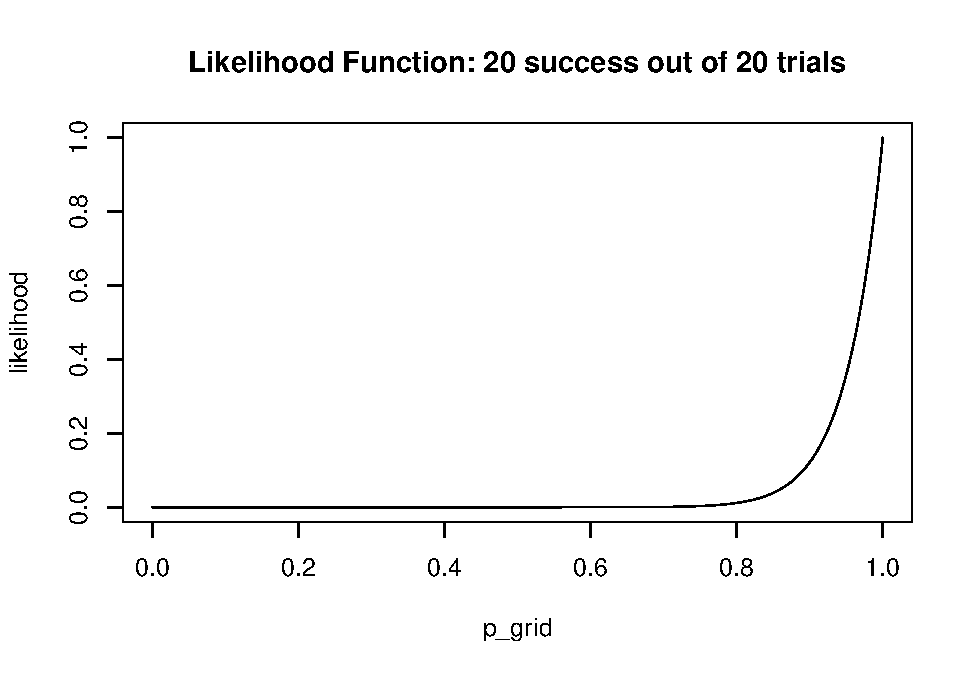
\includegraphics{6_files/figure-latex/unnamed-chunk-5-1} \end{center}

Finally, some quantiles:

\begin{Shaded}
\begin{Highlighting}[]
\CommentTok{# CI for population mean - first column is theta}
\KeywordTok{quantile}\NormalTok{(PHI[, }\DecValTok{1}\NormalTok{], }\KeywordTok{c}\NormalTok{(}\FloatTok{0.025}\NormalTok{, }\FloatTok{0.5}\NormalTok{, }\FloatTok{0.975}\NormalTok{))}
\end{Highlighting}
\end{Shaded}

\begin{verbatim}
##     2.5%      50%    97.5% 
## 1.707282 1.804348 1.901129
\end{verbatim}

\begin{Shaded}
\begin{Highlighting}[]
\CommentTok{# CI for population precision, second column}
\KeywordTok{quantile}\NormalTok{(PHI[, }\DecValTok{2}\NormalTok{], }\KeywordTok{c}\NormalTok{(}\FloatTok{0.025}\NormalTok{, }\FloatTok{0.5}\NormalTok{, }\FloatTok{0.975}\NormalTok{))}
\end{Highlighting}
\end{Shaded}

\begin{verbatim}
##      2.5%       50%     97.5% 
##  17.48020  53.62511 129.20020
\end{verbatim}

\begin{Shaded}
\begin{Highlighting}[]
\CommentTok{# CI for population stddev, arbitrary function of second column}
\KeywordTok{quantile}\NormalTok{(}\DecValTok{1} \OperatorTok{/}\StringTok{ }\KeywordTok{sqrt}\NormalTok{(PHI[, }\DecValTok{2}\NormalTok{]), }\KeywordTok{c}\NormalTok{(}\FloatTok{0.025}\NormalTok{, }\FloatTok{0.5}\NormalTok{, }\FloatTok{0.975}\NormalTok{))}
\end{Highlighting}
\end{Shaded}

\begin{verbatim}
##       2.5%        50%      97.5% 
## 0.08797701 0.13655763 0.23918408
\end{verbatim}

\begin{Shaded}
\begin{Highlighting}[]
\CommentTok{# For later}
\NormalTok{midge.df =}\StringTok{ }\NormalTok{phi.df}
\end{Highlighting}
\end{Shaded}

\hypertarget{general-properties-of-the-gibbs-sampler}{%
\section{General properties of the Gibbs
sampler}\label{general-properties-of-the-gibbs-sampler}}

Under conditions that will be met for our models, like the law of large
numbers for standard monte carlo sampling, a sufficient number of Gibbs
samples approaches the target distribution. The question of course is
how many samples is enough, which is covered in the next section.

Another important point is that Gibbs sampling is not a Bayesian model.
These two concepts should be separated: Gibbs sampling is a general
framework for ``observing'' the posterior probability distribution,
whatever that distribution is.

\hypertarget{introduction-to-mcmc-diagnostics}{%
\section{Introduction to MCMC
diagnostics}\label{introduction-to-mcmc-diagnostics}}

For an example of the importance of assessing convergence of Gibbs
sampling, consider the following target distribution, a 45-10-45 mixture
of \(\mathcal{N}(-3, 1/3), \mathcal{N}(0, 1/3), \mathcal{N}(3, 1/3)\):

\begin{center}\includegraphics{6_files/figure-latex/unnamed-chunk-7-1} \end{center}

A Gibbs sampler to obtain samples from this is:

\begin{Shaded}
\begin{Highlighting}[]
\CommentTok{# Gibbs sampling with S = 1000}
\NormalTok{S =}\StringTok{ }\DecValTok{1000}
\NormalTok{PHI =}\StringTok{ }\KeywordTok{matrix}\NormalTok{(}\DataTypeTok{nrow =}\NormalTok{ S, }\DataTypeTok{ncol =} \DecValTok{2}\NormalTok{)}
\CommentTok{# Let delta0 = 2 and theta0 = 0}
\NormalTok{PHI[}\DecValTok{1}\NormalTok{, ] =}\StringTok{ }\NormalTok{phi =}\StringTok{ }\KeywordTok{c}\NormalTok{(}\DecValTok{2}\NormalTok{, }\DecValTok{0}\NormalTok{)}

\KeywordTok{set.seed}\NormalTok{(}\DecValTok{1}\NormalTok{) }\CommentTok{# Reproducibility}
\CommentTok{# Should use a for loop, as there are variables we need to keep track of through}
\CommentTok{# iterations}
\ControlFlowTok{for}\NormalTok{ (s }\ControlFlowTok{in} \DecValTok{2}\OperatorTok{:}\NormalTok{S) \{}
  \CommentTok{# Sample delta s+1 based on theta s}
\NormalTok{  probs =}\StringTok{ }\KeywordTok{sapply}\NormalTok{(}\DecValTok{1}\OperatorTok{:}\DecValTok{3}\NormalTok{, }\ControlFlowTok{function}\NormalTok{(d) \{}
\NormalTok{    PROB.DENS[d] }\OperatorTok{*}\StringTok{ }\KeywordTok{dnorm}\NormalTok{(phi[}\DecValTok{2}\NormalTok{], MU.DENS[d], }\KeywordTok{sqrt}\NormalTok{(S2.DENS[d]))}
\NormalTok{  \})}
\NormalTok{  probs =}\StringTok{ }\NormalTok{probs }\OperatorTok{/}\StringTok{ }\KeywordTok{sum}\NormalTok{(probs)}
\NormalTok{  phi[}\DecValTok{1}\NormalTok{] =}\StringTok{ }\KeywordTok{sample.int}\NormalTok{(}\DecValTok{3}\NormalTok{, }\DataTypeTok{size =} \DecValTok{1}\NormalTok{, }\DataTypeTok{prob =}\NormalTok{ probs)}

  \CommentTok{# Sample theta s+1 based on delta (easy)}
\NormalTok{  phi[}\DecValTok{2}\NormalTok{] =}\StringTok{ }\KeywordTok{rnorm}\NormalTok{(}\DecValTok{1}\NormalTok{, MU.DENS[phi[}\DecValTok{1}\NormalTok{]], }\KeywordTok{sqrt}\NormalTok{(S2.DENS[phi[}\DecValTok{1}\NormalTok{]]))}

\NormalTok{  PHI[s, ] =}\StringTok{ }\NormalTok{phi}
\NormalTok{\}}

\NormalTok{theta.mcmc =}\StringTok{ }\KeywordTok{data.frame}\NormalTok{(PHI)}
\KeywordTok{colnames}\NormalTok{(theta.mcmc) =}\StringTok{ }\KeywordTok{c}\NormalTok{(}\StringTok{'delta'}\NormalTok{, }\StringTok{'theta'}\NormalTok{)}
\NormalTok{theta.mcmc}\OperatorTok{$}\NormalTok{iteration =}\StringTok{ }\DecValTok{1}\OperatorTok{:}\KeywordTok{nrow}\NormalTok{(theta.mcmc)}

\CommentTok{# How well does this work?}
\KeywordTok{ggplot}\NormalTok{(theta.dist, }\KeywordTok{aes}\NormalTok{(}\DataTypeTok{x =}\NormalTok{ theta, }\DataTypeTok{y =}\NormalTok{ density)) }\OperatorTok{+}
\StringTok{  }\KeywordTok{geom_histogram}\NormalTok{(}\DataTypeTok{mapping =} \KeywordTok{aes}\NormalTok{(}\DataTypeTok{x =}\NormalTok{ theta, }\DataTypeTok{y =}\NormalTok{ ..density..), }\DataTypeTok{data =}\NormalTok{ theta.mcmc,}
                 \DataTypeTok{color =} \StringTok{'black'}\NormalTok{, }\DataTypeTok{fill =} \StringTok{'grey'}\NormalTok{) }\OperatorTok{+}
\StringTok{  }\KeywordTok{geom_line}\NormalTok{()}
\end{Highlighting}
\end{Shaded}

\begin{center}\includegraphics{6_files/figure-latex/unnamed-chunk-8-1} \end{center}

\begin{Shaded}
\begin{Highlighting}[]
\CommentTok{# Traceplot}
\KeywordTok{ggplot}\NormalTok{(theta.mcmc, }\KeywordTok{aes}\NormalTok{(}\DataTypeTok{x =}\NormalTok{ iteration, }\DataTypeTok{y =}\NormalTok{ theta)) }\OperatorTok{+}
\StringTok{  }\KeywordTok{geom_point}\NormalTok{() }\OperatorTok{+}
\StringTok{  }\KeywordTok{geom_line}\NormalTok{(}\DataTypeTok{alpha =} \FloatTok{0.25}\NormalTok{)}
\end{Highlighting}
\end{Shaded}

\begin{center}\includegraphics{6_files/figure-latex/unnamed-chunk-8-2} \end{center}

Notice that the histogram does not adequately approximate the
distribution. Try changing the number of samples to 10000 or 100000,
which should be better.

The problem is that since the sampler generates dependent samples, the
sampler sticks in high probability regions for a long time. After
sufficient samples, this balances out, but sometimes the number of
samples required may be very large.

\hypertarget{getting-it-right}{%
\subsubsection{Getting it right}\label{getting-it-right}}

Estimate of MCMC depends on autocorrelation: how correlated a chain of
values is with itself. We prefer low correlation values. The
\texttt{acf} function can be used to assess this: each bar represents
the autocorrelation for varying levels of lag, where ``lag'' is the gap
in subsequent samples.

\begin{Shaded}
\begin{Highlighting}[]
\KeywordTok{acf}\NormalTok{(theta.mcmc}\OperatorTok{$}\NormalTok{theta, }\DataTypeTok{lag.max =} \DecValTok{50}\NormalTok{)}
\end{Highlighting}
\end{Shaded}

\begin{center}\includegraphics{6_files/figure-latex/unnamed-chunk-9-1} \end{center}

Another thing we can do is obtain the ``effective sample size'' of the
MCMC sample. This exploits the fact that with \(n\) samples of a value
\(\theta\) the following

\begin{align}
\text{Var}_{\text{MCMC}}(\bar{\theta}) = \frac{\text{Var}(\theta)}{n}
\end{align}

only holds if the autocorrelation of the samples is zero. If there is
positive autocorrelation in the samples, the variance of the sample mean
increases, which ``reduces'' \(n\). So by obtaining estimates of the
variance of the population (by estimating the variance of the sample)
and estimates of the variance of the mean, we can solve for \(n\) which
is an ``effective sample size''.

Estimating the variance of the mean, given that we cannot assume an
independent sample, is nontrivial, and requires calculating the
\href{http://faculty.arts.ubc.ca/vmarmer/econ627/627_10_02.pdf}{spectral
density estimate at frequency zero} which is ``a convenient way to
represent the sequence of autocovariances'' of a stochastic process, and
is related to 1) autocorrelation, and 2) Fourier transformation.

This is implemented as the \texttt{effectiveSize} function in R, which
abridged looks like this:

\begin{Shaded}
\begin{Highlighting}[]
\KeywordTok{library}\NormalTok{(coda)}
\NormalTok{myEffectiveSize =}\StringTok{ }\ControlFlowTok{function}\NormalTok{(x) \{}
\NormalTok{    spec =}\StringTok{ }\KeywordTok{spectrum0.ar}\NormalTok{(x)}\OperatorTok{$}\NormalTok{spec}
    \KeywordTok{ifelse}\NormalTok{(spec }\OperatorTok{==}\StringTok{ }\DecValTok{0}\NormalTok{, }\DecValTok{0}\NormalTok{, }\KeywordTok{length}\NormalTok{(x) }\OperatorTok{*}\StringTok{ }\KeywordTok{var}\NormalTok{(x)}\OperatorTok{/}\NormalTok{spec)}
\NormalTok{\}}
\end{Highlighting}
\end{Shaded}

\begin{Shaded}
\begin{Highlighting}[]
\KeywordTok{effectiveSize}\NormalTok{(theta.mcmc}\OperatorTok{$}\NormalTok{theta)}
\end{Highlighting}
\end{Shaded}

\begin{verbatim}
##    var1 
## 5.02999
\end{verbatim}

\begin{Shaded}
\begin{Highlighting}[]
\KeywordTok{myEffectiveSize}\NormalTok{(theta.mcmc}\OperatorTok{$}\NormalTok{theta)}
\end{Highlighting}
\end{Shaded}

\begin{verbatim}
## [1] 5.02999
\end{verbatim}

\hypertarget{mcmc-diagnostics-for-semiconjugate-normal-analysis}{%
\subsubsection{MCMC diagnostics for semiconjugate normal
analysis}\label{mcmc-diagnostics-for-semiconjugate-normal-analysis}}

Back to midge length. Here are the traceplots for our samples of theta
and sigma\^{}2:

\begin{Shaded}
\begin{Highlighting}[]
\NormalTok{midge.df}\OperatorTok{$}\NormalTok{iteration =}\StringTok{ }\NormalTok{midge.df}\OperatorTok{$}\NormalTok{n}
\KeywordTok{ggplot}\NormalTok{(midge.df, }\KeywordTok{aes}\NormalTok{(}\DataTypeTok{x =}\NormalTok{ iteration, }\DataTypeTok{y =}\NormalTok{ theta)) }\OperatorTok{+}
\StringTok{  }\KeywordTok{geom_point}\NormalTok{() }\OperatorTok{+}\StringTok{ }\KeywordTok{geom_line}\NormalTok{(}\DataTypeTok{alpha =} \FloatTok{0.25}\NormalTok{)}
\end{Highlighting}
\end{Shaded}

\begin{center}\includegraphics{6_files/figure-latex/unnamed-chunk-12-1} \end{center}

\begin{Shaded}
\begin{Highlighting}[]
\KeywordTok{ggplot}\NormalTok{(midge.df, }\KeywordTok{aes}\NormalTok{(}\DataTypeTok{x =}\NormalTok{ iteration, }\DataTypeTok{y =} \StringTok{`}\DataTypeTok{1/sigma^2}\StringTok{`}\NormalTok{)) }\OperatorTok{+}
\StringTok{  }\KeywordTok{geom_point}\NormalTok{() }\OperatorTok{+}\StringTok{ }\KeywordTok{geom_line}\NormalTok{(}\DataTypeTok{alpha =} \FloatTok{0.25}\NormalTok{)}
\end{Highlighting}
\end{Shaded}

\begin{center}\includegraphics{6_files/figure-latex/unnamed-chunk-12-2} \end{center}

By viewing the autocorrelation function and effective sample sizes of
our data, we can see that the samples look quite good and seem to have
reasonable effective sample sizes.

\begin{Shaded}
\begin{Highlighting}[]
\KeywordTok{acf}\NormalTok{(midge.df}\OperatorTok{$}\NormalTok{theta)}
\end{Highlighting}
\end{Shaded}

\begin{center}\includegraphics{6_files/figure-latex/unnamed-chunk-13-1} \end{center}

\begin{Shaded}
\begin{Highlighting}[]
\KeywordTok{effectiveSize}\NormalTok{(midge.df}\OperatorTok{$}\NormalTok{theta)}
\end{Highlighting}
\end{Shaded}

\begin{verbatim}
## var1 
## 1000
\end{verbatim}

\begin{Shaded}
\begin{Highlighting}[]
\KeywordTok{acf}\NormalTok{(midge.df}\OperatorTok{$}\StringTok{`}\DataTypeTok{1/sigma^2}\StringTok{`}\NormalTok{)}
\end{Highlighting}
\end{Shaded}

\begin{center}\includegraphics{6_files/figure-latex/unnamed-chunk-13-2} \end{center}

\begin{Shaded}
\begin{Highlighting}[]
\KeywordTok{effectiveSize}\NormalTok{(midge.df}\OperatorTok{$}\StringTok{`}\DataTypeTok{1/sigma^2}\StringTok{`}\NormalTok{)}
\end{Highlighting}
\end{Shaded}

\begin{verbatim}
##     var1 
## 805.4388
\end{verbatim}

\hypertarget{exercises}{%
\section{Exercises}\label{exercises}}

\hypertarget{section}{%
\subsection{6.1}\label{section}}

\hypertarget{a}{%
\subsubsection{a}\label{a}}

\[
\begin{align}
\text{Cov}(\theta_A, \theta_B) &= \mathbb{E}\left[\theta_A \theta_B\right] - \mathbb{E}[\theta_A]\mathbb{E}[\theta_B] \\
&= \mathbb{E}[\theta^2\gamma] - \mathbb{E}[\theta] \mathbb{E}[\theta\gamma] \\
&= \mathbb{E}\left[\theta^2\right] \mathbb{E}\left[ \gamma \right] - \mathbb{E}[\theta]\mathbb{E}[\theta]\mathbb{E}[\gamma] & \theta \perp \gamma \\
&= \mathbb{E}\left[\theta^2\right] \mathbb{E}\left[ \gamma \right] - \mathbb{E}[\theta]^2\mathbb{E}[\gamma] \\
&= \left(\mathbb{E}[\theta^2] - \mathbb{E}[\theta]^2 \right) \mathbb{E}[\gamma] \\
&= \text{Var}(\theta) \mathbb{E}[\gamma] \\
&\neq 0
\end{align}
\]

Since \(\text{Cov}(\theta_A, \theta_B) \neq 0\), \(\theta_A\) and
\(\theta_B\) are dependent.

This prior is justified if we have reason to believe that \(\theta_B\)
is some product of \(\theta_A\) plus random Gamma-distributed noise.

\hypertarget{b}{%
\subsubsection{b}\label{b}}

First the joint posterior distribution

\[
\begin{align}
p(\theta, \gamma \mid \boldsymbol{y}_A, \boldsymbol{y}_B)
&\propto p(\theta, \gamma) \times p(\boldsymbol{y}_A, \boldsymbol{y}_B \mid \theta, \gamma) \\
&= p(\theta) \times p(\gamma) \times p(\boldsymbol{y}_A \mid \theta) \times p(\boldsymbol{y}_B \mid \theta, \gamma) & \boldsymbol{y}_A \perp \gamma \\
&\propto \left(\theta^{a_\theta - 1}e^{-b_\theta \theta}\right) \times \left(\gamma^{a_\gamma - 1}e^{-b_\gamma \gamma} \right) \times  \left(\prod_{i=1}^{n_{A}} \theta^{y_{A_i}} e^{-\theta} \right) \times \left(\prod_{i=1}^{n_{B}} (\gamma \theta)^{y_{B_i}} e^{-\gamma \theta} \right) \\
&= \left(\theta^{a_\theta - 1}e^{-b_\theta \theta}\right) \times \left(\gamma^{a_\gamma - 1}e^{-b_\gamma \gamma} \right) \times  \left( \theta^{\sum_{i = 1}^{n_A} y_{A_i}} e^{-n_A \theta} \right) \times \left( (\gamma \theta)^{\sum_{i=1}^{n_B} y_{B_i}} e^{- n_B \gamma \theta} \right) \\
&= \left(\theta^{a_\theta - 1}e^{-b_\theta \theta}\right) \times \left(\gamma^{a_\gamma - 1}e^{-b_\gamma \gamma} \right) \times  \left( \theta^{n_A \bar{y}_A} e^{-n_A \theta} \right) \times \left( (\gamma \theta)^{n_B \bar{y}_B} e^{- n_B \gamma \theta} \right) \\
\end{align}
\]

So

\[
\begin{align}
p(\theta, \mid \boldsymbol{y}_A, \boldsymbol{y}_B, \gamma)
&\propto \left(\theta^{a_\theta - 1}e^{-b_\theta \theta}\right) \times \left(\gamma^{a_\gamma - 1}e^{-b_\gamma \gamma} \right) \times  \left( \theta^{n_A \bar{y}_A} e^{-n_A \theta} \right) \times \left( (\gamma \theta)^{n_B \bar{y}_B} e^{- n_B \gamma \theta} \right) \\
&\propto \left(\theta^{a_\theta - 1}e^{-b_\theta \theta}\right) \times \left( \theta^{n_A \bar{y}_A} e^{-n_A \theta} \right) \times \left( (\gamma \theta)^{n_B \bar{y}_B} e^{- n_B \gamma \theta} \right) \\
&\propto \theta^{a_\theta + n_A \bar{y}_A + n_B \bar{y}_B - 1} \exp \left( - (b_\theta + n_A + n_B \gamma ) \theta \right) \\
&\propto \text{dgamma}\left(a_\theta + n_A \bar{y}_A + n_B \bar{y}_B, b_\theta + n_A + n_B \gamma \right)
\end{align}
\]

\hypertarget{c}{%
\subsubsection{c}\label{c}}

\[
\begin{align}
p(\gamma, \mid \boldsymbol{y}_A, \boldsymbol{y}_B, \theta)
&\propto \left(\theta^{a_\theta - 1}e^{-b_\theta \theta}\right) \times \left(\gamma^{a_\gamma - 1}e^{-b_\gamma \gamma} \right) \times  \left( \theta^{n_A \bar{y}_A} e^{-n_A \theta} \right) \times \left( (\gamma \theta)^{n_B \bar{y}_B} e^{- n_B \gamma \theta} \right) \\
&\propto \left(\gamma^{a_\gamma - 1}e^{-b_\gamma \gamma} \right) \times \left( (\gamma \theta)^{n_B \bar{y}_B} e^{- n_B \gamma \theta} \right) \\
&\propto \left(\gamma^{a_\gamma - 1}e^{-b_\gamma \gamma} \right) \times \left( \gamma^{n_B \bar{y}_B} e^{- n_B \gamma \theta} \right) \\
&\propto \gamma^{a_\gamma + n_B \bar{y}_B - 1} \exp\left( -(b_\gamma + n_B \theta) \gamma \right) \\
&\propto \text{dgamma}\left(a_\gamma + n_B\bar{y}_B, b_\gamma + n_B \theta \right)
\end{align}
\]

\hypertarget{d}{%
\subsubsection{d}\label{d}}

\begin{Shaded}
\begin{Highlighting}[]
\NormalTok{Y_a <-}\StringTok{ }\KeywordTok{scan}\NormalTok{(}\KeywordTok{url}\NormalTok{(}\StringTok{'http://www.stat.washington.edu/~pdhoff/Book/Data/hwdata/menchild30bach.dat'}\NormalTok{))}
\NormalTok{Y_b <-}\StringTok{ }\KeywordTok{scan}\NormalTok{(}\KeywordTok{url}\NormalTok{(}\StringTok{'http://www.stat.washington.edu/~pdhoff/Book/Data/hwdata/menchild30nobach.dat'}\NormalTok{))}
\NormalTok{n_a =}\StringTok{ }\KeywordTok{length}\NormalTok{(Y_a)}
\NormalTok{n_b =}\StringTok{ }\KeywordTok{length}\NormalTok{(Y_b)}
\NormalTok{ybar_a =}\StringTok{ }\KeywordTok{mean}\NormalTok{(Y_a)}
\NormalTok{ybar_b =}\StringTok{ }\KeywordTok{mean}\NormalTok{(Y_b)}

\NormalTok{a_theta =}\StringTok{ }\DecValTok{2}
\NormalTok{b_theta =}\StringTok{ }\DecValTok{1}

\NormalTok{S =}\StringTok{ }\DecValTok{5000}

\NormalTok{ab_gamma =}\StringTok{ }\KeywordTok{c}\NormalTok{(}\DecValTok{8}\NormalTok{, }\DecValTok{16}\NormalTok{, }\DecValTok{32}\NormalTok{, }\DecValTok{64}\NormalTok{, }\DecValTok{128}\NormalTok{)}

\NormalTok{theta_diff =}\StringTok{ }\KeywordTok{sapply}\NormalTok{(ab_gamma, }\ControlFlowTok{function}\NormalTok{(abg) \{}
\NormalTok{  a_gamma =}\StringTok{ }\NormalTok{b_gamma =}\StringTok{ }\NormalTok{abg}

\NormalTok{  THETA =}\StringTok{ }\KeywordTok{numeric}\NormalTok{(S)}
\NormalTok{  GAMMA =}\StringTok{ }\KeywordTok{numeric}\NormalTok{(S)}

  \CommentTok{# Starting values}
\NormalTok{  theta =}\StringTok{ }\NormalTok{ybar_a}
\NormalTok{  gamma =}\StringTok{ }\NormalTok{ybar_a }\OperatorTok{/}\StringTok{ }\NormalTok{ybar_b  }\CommentTok{# Relative rate \textbackslash{}theta_B / \textbackslash{}theta_A}

  \ControlFlowTok{for}\NormalTok{ (s }\ControlFlowTok{in} \DecValTok{1}\OperatorTok{:}\NormalTok{S) \{}
    \CommentTok{# Sample theta \textbackslash{}text\{dgamma\}\textbackslash{}left(a_\textbackslash{}theta + n_A \textbackslash{}bar\{y\}_A + n_B \textbackslash{}bar\{y\}_B, b_\textbackslash{}theta + n_A + n_B \textbackslash{}gamma \textbackslash{}right)}
\NormalTok{    theta =}\StringTok{ }\KeywordTok{rgamma}\NormalTok{(}
      \DecValTok{1}\NormalTok{,}
\NormalTok{      a_theta }\OperatorTok{+}\StringTok{ }\NormalTok{n_a }\OperatorTok{*}\StringTok{ }\NormalTok{ybar_a }\OperatorTok{+}\StringTok{ }\NormalTok{n_b }\OperatorTok{*}\StringTok{ }\NormalTok{ybar_b,}
\NormalTok{      b_theta }\OperatorTok{+}\StringTok{ }\NormalTok{n_a }\OperatorTok{+}\StringTok{ }\NormalTok{n_b }\OperatorTok{*}\StringTok{ }\NormalTok{gamma}
\NormalTok{    )}

    \CommentTok{# Sample gamma from \textbackslash{}text\{dgamma\}\textbackslash{}left(a_\textbackslash{}gamma + n_B\textbackslash{}bar\{y\}_B, b_\textbackslash{}gamma + n_B \textbackslash{}theta \textbackslash{}right)}
\NormalTok{    gamma =}\StringTok{ }\KeywordTok{rgamma}\NormalTok{(}
      \DecValTok{1}\NormalTok{,}
\NormalTok{      a_gamma }\OperatorTok{+}\StringTok{ }\NormalTok{n_b }\OperatorTok{*}\StringTok{ }\NormalTok{ybar_b,}
\NormalTok{      b_gamma }\OperatorTok{+}\StringTok{ }\NormalTok{n_b }\OperatorTok{*}\StringTok{ }\NormalTok{theta}
\NormalTok{    )}

\NormalTok{    THETA[s] =}\StringTok{ }\NormalTok{theta}
\NormalTok{    GAMMA[s] =}\StringTok{ }\NormalTok{gamma}
\NormalTok{  \}}

  \CommentTok{# Reconstruct \textbackslash{}theta_A, \textbackslash{}theta_B}
\NormalTok{  THETA_A =}\StringTok{ }\NormalTok{THETA}
\NormalTok{  THETA_B =}\StringTok{ }\NormalTok{THETA }\OperatorTok{*}\StringTok{ }\NormalTok{GAMMA}

  \KeywordTok{mean}\NormalTok{(THETA_B }\OperatorTok{-}\StringTok{ }\NormalTok{THETA_A)}
\NormalTok{\})}

\KeywordTok{ggplot}\NormalTok{(}\KeywordTok{data.frame}\NormalTok{(}\DataTypeTok{ab_gamma =}\NormalTok{ ab_gamma, }\DataTypeTok{theta_diff =}\NormalTok{ theta_diff), }\KeywordTok{aes}\NormalTok{(}\DataTypeTok{x =}\NormalTok{ ab_gamma, }\DataTypeTok{y =}\NormalTok{ theta_diff)) }\OperatorTok{+}
\StringTok{  }\KeywordTok{geom_point}\NormalTok{() }\OperatorTok{+}
\StringTok{  }\KeywordTok{geom_line}\NormalTok{()}
\end{Highlighting}
\end{Shaded}

\begin{center}\includegraphics{6_files/figure-latex/unnamed-chunk-14-1} \end{center}

Since \(a_\gamma\) and \(b_\gamma\) are equal, the gamma distribution is
centered around 1 and the magnitude represents the strength of our
belief that \(\gamma\) (the proportion \(\theta_B / \theta_A\)) is 1. As
expected, as our belief in that increases, the mean posterior difference
between \(\theta_B\) and \(\theta_A\) decreases.

\hypertarget{section-1}{%
\subsection{6.2}\label{section-1}}

\begin{Shaded}
\begin{Highlighting}[]
\NormalTok{glucose <-}\StringTok{ }\KeywordTok{scan}\NormalTok{(}\KeywordTok{url}\NormalTok{(}\StringTok{'http://www.stat.washington.edu/~pdhoff/Book/Data/hwdata/glucose.dat'}\NormalTok{))}
\end{Highlighting}
\end{Shaded}

\hypertarget{a-1}{%
\subsubsection{a}\label{a-1}}

\begin{Shaded}
\begin{Highlighting}[]
\KeywordTok{qplot}\NormalTok{(glucose, }\DataTypeTok{geom =} \StringTok{'histogram'}\NormalTok{)}
\end{Highlighting}
\end{Shaded}

\begin{center}\includegraphics{6_files/figure-latex/unnamed-chunk-16-1} \end{center}

Appears to be skewed right significantly.

\hypertarget{b-1}{%
\subsubsection{b}\label{b-1}}

The likelihood is

\[
\begin{align}
p(\boldsymbol{y} \mid \boldsymbol{x}, p, \theta_1, \theta_2, \sigma^2_1, \sigma^2_2) &= 
\prod_{i = 1}^n p(y_i \mid x_i, p, \theta_1, \theta_2, \sigma^2_1, \sigma^2_2) \\
&= \prod_{i = 1}^n \text{dnorm}(y_i, \theta_1, \sigma^2_1)^{x_i} \text{dnorm}(y_i, \theta_2, \sigma^2_2)^{1 - x_i} \\
\end{align}
\]

\hypertarget{boldsymbolx}{%
\paragraph{\texorpdfstring{\(\boldsymbol{x}\)}{\textbackslash{}boldsymbol\{x\}}}\label{boldsymbolx}}

First observe the probability that a single \(X_i = 1\):

\[
\begin{align}
P(X_i = 1 \mid y_i, p, \theta_1, \theta_2, \sigma^2_1, \sigma^2_2) &= \frac{P(X_i = 1 \mid p, \theta_1, \theta_2, \sigma^2_1, \sigma^2_2) \times p(y_i \mid X_i = 1, p, \theta_1, \theta_2, \sigma^2_1, \sigma^2_2)}{P(y_i \mid p, \theta_1, \theta_2, \sigma^2_1, \sigma^2_2)} \\
&=
\frac{P(X_i = 1 \mid p) \times p(y_i \mid X_i = 1, \theta_1, \sigma^2_1)}{P(X_i = 1 \mid p) \times p(y_i \mid X_i = 1, \theta_1, \sigma^2_1) + P(X_i = 0 \mid p) \times p(y_i \mid X_i = 0, \theta_2, \sigma^2_2)} \\
&= \frac{p \times \text{dnorm}(y_i, \theta_1, \sigma^2_1)}{p \times \text{dnorm}(y_i, \theta_1, \sigma^2_1) + (1 - p) \times \text{dnorm}(y_i, \theta_2, \sigma^2_2)}
\end{align}
\]

Since this is similar for \(P(X_i = 0)\), we know

\[
x_i \sim \text{Bernoulli}\left(\frac{p \times \text{dnorm}(y_i, \theta_1, \sigma^2_1)}{p \times \text{dnorm}(y_i, \theta_1, \sigma^2_1) + (1 - p) \times \text{dnorm}(y_i, \theta_2, \sigma^2_2)}\right)
\]

\hypertarget{p}{%
\paragraph{\texorpdfstring{\(p\)}{p}}\label{p}}

For this and later calculations, let \(n_1 = \sum x_i\) (i.e.~number of
1s in \(\boldsymbol{x}\)) and \(n_2 = n - n_1\) (i.e.~number of 0s).

\[
\begin{align}
p(p \mid \boldsymbol{x}, \boldsymbol{y}, \theta_1, \theta_2, \sigma^2_1, \sigma^2_2) &\propto p(p) \times p(\boldsymbol{x}, \boldsymbol{y}, \theta_1, \theta_2, \sigma^2_1, \sigma^2_2 \mid p) \\
&\propto p(p) \times p(\boldsymbol{x} \mid p) p(\boldsymbol{y} \mid \boldsymbol{x}, \theta_1, \theta_2, \sigma^2_1, \sigma^2_2) p(\theta_1, \theta_2, \sigma^2_1, \sigma^2_2) \\
&\propto p(p) \times p(\boldsymbol{x} \mid p) \\
&\propto \text{dbeta}(p, a, b) \times \text{dbinom}(n_1, n, p) \\
&\propto p^{a - 1} (1 - p)^{b - 1} \times p^{n_1} (1 - p)^{n_2} \\
&= p^{a + n_1 - 1}(1 - p)^{b + n_2 - 1} \\
&= \text{dbeta}(p, a + n_1, b + n_2)
\end{align}
\]

\hypertarget{theta_1}{%
\paragraph{\texorpdfstring{\(\theta_1\)}{\textbackslash{}theta\_1}}\label{theta_1}}

Let \(\boldsymbol{y}_1 = \{y_i \in \boldsymbol{y} \; : \; x_i = 1 \}\)
and \(\boldsymbol{y}_2 = \{y_i \in \boldsymbol{y} \; : \; x_i = 0 \}\)

\[
\begin{align}
p(\theta_1 \mid \boldsymbol{x}, \boldsymbol{y}, p, \theta_2, \sigma^2_1, \sigma^2_2) &\propto p(\theta_1 \mid \boldsymbol{x}, p, \theta_2, \sigma^2_1, \sigma^2_2) \times p(\boldsymbol{y} \mid \boldsymbol{x}, p, \theta_1, \theta_2, \sigma^2_1, \sigma^2_2) \\
&\propto p(\theta_1) \times \prod_{i=1}^n \left( \text{dnorm}(y_i, \theta_1, \sigma^2_1)^{x_i} \text{dnorm}(y_i, \theta_2, \sigma^2_2)^{1 - x_i} \right) \\
&\propto \text{dnorm}(\theta_1, \mu_0, \tau^2_0) \times \prod_{i = 1}^n \text{dnorm}(y_i, \theta_1, \sigma^2_1)^{x_i} \\
&\propto \text{dnorm}(\theta_1, \mu_0, \tau^2_0) \times \prod_{y \in \boldsymbol{y}_1} \text{dnorm}(y, \theta_1, \sigma^2_1) \\
&\propto \exp \left(- \frac{1}{2 \tau^2_0} (\theta_1 - \mu_0)^2 \right) \times \prod_{y \in \boldsymbol{y}_1} \exp\left( -\frac{1}{2\sigma^2_1} (y - \theta_1)^2\right) \\
&\propto \exp \left(- \frac{1}{2 \tau^2_0} (\theta_1 - \mu_0)^2 \right) \times \exp\left(-\frac{1}{2\sigma^2_1} \sum_{y \in \boldsymbol{y}_1} (y - \theta_1)^2 \right) \\
&\propto \text{calculations from 5.2...} \\
&\propto \mathcal{N}(\tau^2_{n , 1}, \mu_{n, 1})
\end{align}
\]

where

\[
\begin{align}
\tau^2_{n, 1} &= \frac{1}{\frac{1}{\tau^2_0} + \frac{n_1}{\sigma^2_1}} \\
\mu_{n, 1} &= \frac{\frac{1}{\tau^2_0}\mu_0 + \frac{n_1}{\sigma^2_1} \bar{y}_{\cdot, 1}}{\frac{1}{\tau^2_0} + \frac{n_1}{\sigma^2_1}}
\end{align}
\]

\hypertarget{theta_2}{%
\paragraph{\texorpdfstring{\(\theta_2\)}{\textbackslash{}theta\_2}}\label{theta_2}}

\(\theta_2 \mid \dots \sim \mathcal{N}(\mu_{n, 2}, \tau^2_{n, 2})\) like
\(\theta_1\) but with the subscripts switched from 1 to 2.

\hypertarget{sigma2_1}{%
\paragraph{\texorpdfstring{\(\sigma^2_1\)}{\textbackslash{}sigma\^{}2\_1}}\label{sigma2_1}}

As probably expected, this will look like inference for a standard
normal model, except using only the data in group 1.

\[
\begin{align}
p(\sigma^2_1 \mid \boldsymbol{x}, \boldsymbol{y}, p, \theta_1, \theta_2, \sigma^2_2) &\propto p(\sigma^2_1 \mid \boldsymbol{x}, p, \theta_1, \theta_2, \sigma^2_2) \times p(\boldsymbol{y} \mid \boldsymbol{x}, p, \theta_1, \theta_2, \sigma^2_1, \sigma^2_2) \\
&\propto p(\sigma^2_1) \times \prod_{i=1}^n \left( \text{dnorm}(y_i, \theta_1, \sigma^2_1)^{x_i} \text{dnorm}(y_i, \theta_2, \sigma^2_2)^{1 - x_i} \right) \\
&\propto \text{inverse-gamma}(\sigma^2_1, \nu_0, \sigma^2_0 \nu_0 / 2) \times \prod_{y \in \boldsymbol{y}_1} \text{dnorm}(y, \theta_1, \sigma^2_1) \\
&\propto \exp \left((\sigma_1^2)^{-(\nu_0 / 2) - 1} \exp\left( -\frac{1}{\sigma^2_1} \sigma^2_0 \nu_0 / 2 \right) \right) \times (\sigma_1^2)^{-n / 2} \exp\left(-\frac{1}{2\sigma^2_1} \sum_{y \in \boldsymbol{y}_1} (y - \theta_1)^2 \right) \\
&\propto \text{calculations from 6.3...} \\
&\propto \text{inverse-gamma}(\nu_{n, 1} / 2, \sigma^2_{n, 1}(\theta_1) \nu_{n, 1} / 2)
\end{align}
\]

where

\[
\begin{align}
\nu_{n, 1} &= \nu_0 + n_1 \\
\sigma^2_{n, 1}(\theta_1) &= \frac{1}{\nu_{n, 1}} \left[\nu_0 \sigma^2_0 + n_1 s^2_{n, 1}(\theta_1) \right]
\end{align}
\]

\hypertarget{sigma2_2}{%
\paragraph{\texorpdfstring{\(\sigma^2_2\)}{\textbackslash{}sigma\^{}2\_2}}\label{sigma2_2}}

Same as above, but with subscripts switched.

\hypertarget{c-1}{%
\subsubsection{c}\label{c-1}}

\begin{Shaded}
\begin{Highlighting}[]
\NormalTok{Y =}\StringTok{ }\NormalTok{glucose}
\NormalTok{n =}\StringTok{ }\KeywordTok{length}\NormalTok{(Y)}

\CommentTok{# Priors}
\NormalTok{a =}\StringTok{ }\NormalTok{b =}\StringTok{ }\DecValTok{1}
\NormalTok{mu0 =}\StringTok{ }\DecValTok{120}
\NormalTok{t20 =}\StringTok{ }\DecValTok{200}
\NormalTok{s20 =}\StringTok{ }\DecValTok{1000}
\NormalTok{nu0 =}\StringTok{ }\DecValTok{10}

\NormalTok{S =}\StringTok{ }\DecValTok{10000}

\CommentTok{# Values we'd like to store. Don't care about xs, p, sigmas}
\NormalTok{THETA1 =}\StringTok{ }\KeywordTok{numeric}\NormalTok{(S)}
\NormalTok{THETA2 =}\StringTok{ }\KeywordTok{numeric}\NormalTok{(S)}
\NormalTok{YPRED =}\StringTok{ }\KeywordTok{numeric}\NormalTok{(S) }\CommentTok{# Posterior predictive}

\CommentTok{# Starting values}
\NormalTok{p =}\StringTok{ }\FloatTok{0.5}
\NormalTok{theta1 =}\StringTok{ }\NormalTok{theta2 =}\StringTok{ }\KeywordTok{mean}\NormalTok{(Y)}
\NormalTok{s21 =}\StringTok{ }\NormalTok{s22 =}\StringTok{ }\KeywordTok{var}\NormalTok{(Y)}

\CommentTok{# Gibbs sampling}
\ControlFlowTok{for}\NormalTok{ (s }\ControlFlowTok{in} \DecValTok{1}\OperatorTok{:}\NormalTok{S) \{}
  \CommentTok{# Sample X}
  \CommentTok{# We calculate dnorm for each y so p1 and p2 are vectors}
\NormalTok{  p1 =}\StringTok{ }\NormalTok{p }\OperatorTok{*}\StringTok{ }\KeywordTok{dnorm}\NormalTok{(Y, theta1, }\KeywordTok{sqrt}\NormalTok{(s21))}
\NormalTok{  p2 =}\StringTok{ }\NormalTok{(}\DecValTok{1} \OperatorTok{-}\StringTok{ }\NormalTok{p) }\OperatorTok{*}\StringTok{ }\KeywordTok{dnorm}\NormalTok{(Y, theta2, }\KeywordTok{sqrt}\NormalTok{(s22))}
\NormalTok{  bernoulli_p =}\StringTok{ }\NormalTok{p1 }\OperatorTok{/}\StringTok{ }\NormalTok{(p1 }\OperatorTok{+}\StringTok{ }\NormalTok{p2)}
\NormalTok{  X =}\StringTok{ }\KeywordTok{rbinom}\NormalTok{(n, }\DecValTok{1}\NormalTok{, bernoulli_p)}
  
  \CommentTok{# With X sample, calcuate group-specific summary statistics}
\NormalTok{  n1 =}\StringTok{ }\KeywordTok{sum}\NormalTok{(X)}
\NormalTok{  n2 =}\StringTok{ }\NormalTok{n }\OperatorTok{-}\StringTok{ }\NormalTok{n1}
\NormalTok{  y1 =}\StringTok{ }\NormalTok{Y[X }\OperatorTok{==}\StringTok{ }\DecValTok{1}\NormalTok{]}
\NormalTok{  y2 =}\StringTok{ }\NormalTok{Y[X }\OperatorTok{==}\StringTok{ }\DecValTok{0}\NormalTok{]}
\NormalTok{  ybar1 =}\StringTok{ }\KeywordTok{mean}\NormalTok{(y1)}
\NormalTok{  ybar2 =}\StringTok{ }\KeywordTok{mean}\NormalTok{(y2)}
\NormalTok{  yvar1 =}\StringTok{ }\KeywordTok{var}\NormalTok{(y1)}
\NormalTok{  yvar2 =}\StringTok{ }\KeywordTok{var}\NormalTok{(y2)}
  
  \CommentTok{# Sample p}
\NormalTok{  p =}\StringTok{ }\KeywordTok{rbeta}\NormalTok{(}\DecValTok{1}\NormalTok{, a }\OperatorTok{+}\StringTok{ }\NormalTok{n1, b }\OperatorTok{+}\StringTok{ }\NormalTok{n2)}
  
  \CommentTok{# Sample thetas}
\NormalTok{  t2n1 =}\StringTok{ }\DecValTok{1} \OperatorTok{/}\StringTok{ }\NormalTok{(}\DecValTok{1} \OperatorTok{/}\StringTok{ }\NormalTok{t20 }\OperatorTok{+}\StringTok{ }\NormalTok{n1 }\OperatorTok{/}\StringTok{ }\NormalTok{s21)}
\NormalTok{  mun1 =}\StringTok{ }\NormalTok{(mu0 }\OperatorTok{/}\StringTok{ }\NormalTok{t20 }\OperatorTok{+}\StringTok{ }\NormalTok{n1 }\OperatorTok{*}\StringTok{ }\NormalTok{ybar1 }\OperatorTok{/}\StringTok{ }\NormalTok{s21) }\OperatorTok{/}\StringTok{ }\NormalTok{(}\DecValTok{1} \OperatorTok{/}\StringTok{ }\NormalTok{t20 }\OperatorTok{+}\StringTok{ }\NormalTok{n1 }\OperatorTok{/}\StringTok{ }\NormalTok{s21)}
\NormalTok{  theta1 =}\StringTok{ }\KeywordTok{rnorm}\NormalTok{(}\DecValTok{1}\NormalTok{, mun1, }\KeywordTok{sqrt}\NormalTok{(t2n1))}
  
\NormalTok{  t2n2 =}\StringTok{ }\DecValTok{1} \OperatorTok{/}\StringTok{ }\NormalTok{(}\DecValTok{1} \OperatorTok{/}\StringTok{ }\NormalTok{t20 }\OperatorTok{+}\StringTok{ }\NormalTok{n2 }\OperatorTok{/}\StringTok{ }\NormalTok{s22)}
\NormalTok{  mun2 =}\StringTok{ }\NormalTok{(mu0 }\OperatorTok{/}\StringTok{ }\NormalTok{t20 }\OperatorTok{+}\StringTok{ }\NormalTok{n2 }\OperatorTok{*}\StringTok{ }\NormalTok{ybar2 }\OperatorTok{/}\StringTok{ }\NormalTok{s22) }\OperatorTok{/}\StringTok{ }\NormalTok{(}\DecValTok{1} \OperatorTok{/}\StringTok{ }\NormalTok{t20 }\OperatorTok{+}\StringTok{ }\NormalTok{n2 }\OperatorTok{/}\StringTok{ }\NormalTok{s22)}
\NormalTok{  theta2 =}\StringTok{ }\KeywordTok{rnorm}\NormalTok{(}\DecValTok{1}\NormalTok{, mun2, }\KeywordTok{sqrt}\NormalTok{(t2n2))}

  \CommentTok{# Sample sigma^2s}
\NormalTok{  nun1 =}\StringTok{ }\NormalTok{nu0 }\OperatorTok{+}\StringTok{ }\NormalTok{n1}
\NormalTok{  s2n1 =}\StringTok{ }\NormalTok{(nu0 }\OperatorTok{*}\StringTok{ }\NormalTok{s20 }\OperatorTok{+}\StringTok{ }\NormalTok{(n1 }\OperatorTok{-}\StringTok{ }\DecValTok{1}\NormalTok{) }\OperatorTok{*}\StringTok{ }\NormalTok{yvar1 }\OperatorTok{+}\StringTok{ }\NormalTok{n1 }\OperatorTok{*}\StringTok{ }\NormalTok{(ybar1 }\OperatorTok{-}\StringTok{ }\NormalTok{theta1)}\OperatorTok{^}\DecValTok{2}\NormalTok{) }\OperatorTok{/}\StringTok{ }\NormalTok{nun1}
\NormalTok{  s21 =}\StringTok{ }\DecValTok{1} \OperatorTok{/}\StringTok{ }\KeywordTok{rgamma}\NormalTok{(}\DecValTok{1}\NormalTok{, nun1 }\OperatorTok{/}\StringTok{ }\DecValTok{2}\NormalTok{, s2n1 }\OperatorTok{*}\StringTok{ }\NormalTok{nun1 }\OperatorTok{/}\StringTok{ }\DecValTok{2}\NormalTok{)}

\NormalTok{  nun2 =}\StringTok{ }\NormalTok{nu0 }\OperatorTok{+}\StringTok{ }\NormalTok{n2}
\NormalTok{  s2n2 =}\StringTok{ }\NormalTok{(nu0 }\OperatorTok{*}\StringTok{ }\NormalTok{s20 }\OperatorTok{+}\StringTok{ }\NormalTok{(n2 }\OperatorTok{-}\StringTok{ }\DecValTok{1}\NormalTok{) }\OperatorTok{*}\StringTok{ }\NormalTok{yvar2 }\OperatorTok{+}\StringTok{ }\NormalTok{n2 }\OperatorTok{*}\StringTok{ }\NormalTok{(ybar2 }\OperatorTok{-}\StringTok{ }\NormalTok{theta2)}\OperatorTok{^}\DecValTok{2}\NormalTok{) }\OperatorTok{/}\StringTok{ }\NormalTok{nun2}
\NormalTok{  s22 =}\StringTok{ }\DecValTok{1} \OperatorTok{/}\StringTok{ }\KeywordTok{rgamma}\NormalTok{(}\DecValTok{1}\NormalTok{, nun2 }\OperatorTok{/}\StringTok{ }\DecValTok{2}\NormalTok{, s2n2 }\OperatorTok{*}\StringTok{ }\NormalTok{nun2 }\OperatorTok{/}\StringTok{ }\DecValTok{2}\NormalTok{)}
  
  \CommentTok{# Sample posterior predictive}
\NormalTok{  xpred =}\StringTok{ }\KeywordTok{runif}\NormalTok{(}\DecValTok{1}\NormalTok{) }\OperatorTok{<}\StringTok{ }\NormalTok{p}
\NormalTok{  ypred =}\StringTok{ }\KeywordTok{ifelse}\NormalTok{(xpred, }\KeywordTok{rnorm}\NormalTok{(}\DecValTok{1}\NormalTok{, theta1, }\KeywordTok{sqrt}\NormalTok{(s21)), }\KeywordTok{rnorm}\NormalTok{(}\DecValTok{1}\NormalTok{, theta2, }\KeywordTok{sqrt}\NormalTok{(s22)))}
  
  \CommentTok{# Store values}
\NormalTok{  THETA1[s] =}\StringTok{ }\NormalTok{theta1}
\NormalTok{  THETA2[s] =}\StringTok{ }\NormalTok{theta2}
\NormalTok{  YPRED[s] =}\StringTok{ }\NormalTok{ypred}
\NormalTok{\}}
\end{Highlighting}
\end{Shaded}

\begin{Shaded}
\begin{Highlighting}[]
\NormalTok{THETAMIN =}\StringTok{ }\KeywordTok{pmin}\NormalTok{(THETA1, THETA2)}
\NormalTok{THETAMAX =}\StringTok{ }\KeywordTok{pmax}\NormalTok{(THETA1, THETA2)}

\KeywordTok{library}\NormalTok{(coda)}

\KeywordTok{acf}\NormalTok{(THETAMIN)}
\end{Highlighting}
\end{Shaded}

\begin{center}\includegraphics{6_files/figure-latex/unnamed-chunk-18-1} \end{center}

\begin{Shaded}
\begin{Highlighting}[]
\KeywordTok{effectiveSize}\NormalTok{(THETAMIN)}
\end{Highlighting}
\end{Shaded}

\begin{verbatim}
##     var1 
## 534.7286
\end{verbatim}

\begin{Shaded}
\begin{Highlighting}[]
\KeywordTok{acf}\NormalTok{(THETAMAX)}
\end{Highlighting}
\end{Shaded}

\begin{center}\includegraphics{6_files/figure-latex/unnamed-chunk-18-2} \end{center}

\begin{Shaded}
\begin{Highlighting}[]
\KeywordTok{effectiveSize}\NormalTok{(THETAMAX)}
\end{Highlighting}
\end{Shaded}

\begin{verbatim}
##     var1 
## 227.5474
\end{verbatim}

These samples are actually highly autocorrelated, hence the minimum
effective sample sizes. But I'm not sure (?) the purpose of calculating
the autocorrelation of the minimum and maximum \(\theta\)?

\hypertarget{d-1}{%
\subsubsection{d}\label{d-1}}

\begin{Shaded}
\begin{Highlighting}[]
\NormalTok{YCOMP =}\StringTok{ }\KeywordTok{rbind}\NormalTok{(}\KeywordTok{data.frame}\NormalTok{(}\DataTypeTok{y =}\NormalTok{ YPRED, }\DataTypeTok{dataset =} \StringTok{'predictive'}\NormalTok{), }\KeywordTok{data.frame}\NormalTok{(}\DataTypeTok{y =}\NormalTok{ Y, }\DataTypeTok{dataset =} \StringTok{'original'}\NormalTok{))}
\KeywordTok{ggplot}\NormalTok{(YCOMP, }\KeywordTok{aes}\NormalTok{(}\DataTypeTok{x =}\NormalTok{ y, }\DataTypeTok{fill =}\NormalTok{ dataset)) }\OperatorTok{+}
\StringTok{  }\KeywordTok{geom_density}\NormalTok{(}\DataTypeTok{alpha =} \FloatTok{0.5}\NormalTok{)}
\end{Highlighting}
\end{Shaded}

\begin{center}\includegraphics{6_files/figure-latex/unnamed-chunk-19-1} \end{center}

Based on the very close correspondence with the densities of the
original and posterior predictive dataset, it seems like this mixture
model fits very well.


\end{document}
